\documentclass[a4paper]{report}
\usepackage{bbold}
\usepackage[a4paper, total={6in, 10in}]{geometry}
% basics
\usepackage[utf8]{inputenc}
\usepackage[T1]{fontenc}
\usepackage{textcomp}
% \usepackage[dutch]{babel}
\usepackage{url}
% \usepackage{hyperref}
% \hypersetup{
%     colorlinks,
%     linkcolor={black},
%     citecolor={black},
%     urlcolor={blue!80!black}
% }
\usepackage{graphicx}
\usepackage{float}
\usepackage{booktabs}
\usepackage{enumitem}
% \usepackage{parskip}
\usepackage{emptypage}
\usepackage{subcaption}
\usepackage{multicol}
\usepackage[usenames,dvipsnames]{xcolor}

% \usepackage{cmbright}


\usepackage{amsmath, amsfonts, mathtools, amsthm, amssymb}
\usepackage{mathrsfs}
\usepackage{cancel}
\usepackage{bm}
\newcommand\N{\ensuremath{\mathbb{N}}}
\newcommand\R{\ensuremath{\mathbb{R}}}
\newcommand\Z{\ensuremath{\mathbb{Z}}}
\renewcommand\O{\ensuremath{\emptyset}}
\newcommand\Q{\ensuremath{\mathbb{Q}}}
\newcommand\C{\ensuremath{\mathbb{C}}}
\DeclareMathOperator{\sgn}{sgn}
\usepackage{systeme}
\let\svlim\lim\def\lim{\svlim\limits}
\let\implies\Rightarrow
\let\impliedby\Leftarrow
\let\iff\Leftrightarrow
\let\epsilon\varepsilon
\usepackage{stmaryrd} % for \lightning
\newcommand\contra{\scalebox{1.1}{$\lightning$}}
% \let\phi\varphi





% correct
\definecolor{correct}{HTML}{009900}
\newcommand\correct[2]{\ensuremath{\:}{\color{red}{#1}}\ensuremath{\to }{\color{correct}{#2}}\ensuremath{\:}}
\newcommand\green[1]{{\color{correct}{#1}}}



% horizontal rule
\newcommand\hr{
    \noindent\rule[0.5ex]{\linewidth}{0.5pt}
}


% hide parts
\newcommand\hide[1]{}



% si unitx
\usepackage{siunitx}
\sisetup{locale = FR}
% \renewcommand\vec[1]{\mathbf{#1}}
\newcommand\mat[1]{\mathbf{#1}}


% tikz
\usepackage{tikz}
\usepackage{tikz-qtree}
\usepackage{tikz-cd}
\usetikzlibrary{intersections, angles, quotes, calc, positioning, backgrounds,matrix}
\usetikzlibrary{arrows.meta}
\usepackage{pgfplots}
\pgfplotsset{compat=1.13}


\tikzset{
    force/.style={thick, {Circle[length=2pt]}-stealth, shorten <=-1pt}
}

% theorems
\makeatother
\usepackage{thmtools}
\usepackage[framemethod=TikZ]{mdframed}
\mdfsetup{skipabove=1em,skipbelow=0em}


\theoremstyle{definition}

\declaretheoremstyle[
    headfont=\bfseries\sffamily\color{ForestGreen!70!black}, bodyfont=\normalfont,
    mdframed={
        linewidth=2pt,
        rightline=false, topline=false, bottomline=false,
        linecolor=ForestGreen, backgroundcolor=ForestGreen!5,
    }
]{thmgreenbox}

\declaretheoremstyle[
    headfont=\bfseries\sffamily\color{NavyBlue!70!black}, bodyfont=\normalfont,
    mdframed={
        linewidth=2pt,
        rightline=false, topline=false, bottomline=false,
        linecolor=NavyBlue, backgroundcolor=NavyBlue!5,
    }
]{thmbluebox}

\declaretheoremstyle[
    headfont=\bfseries\sffamily\color{NavyBlue!70!black}, bodyfont=\normalfont,
    mdframed={
        linewidth=2pt,
        rightline=false, topline=false, bottomline=false,
        linecolor=NavyBlue
    }
]{thmblueline}

\declaretheoremstyle[
    headfont=\bfseries\sffamily\color{RawSienna!70!black}, bodyfont=\normalfont,
    mdframed={
        linewidth=2pt,
        rightline=false, topline=false, bottomline=false,
        linecolor=RawSienna, backgroundcolor=RawSienna!5,
    }
]{thmredbox}

\declaretheoremstyle[
    headfont=\bfseries\sffamily\color{RawSienna!70!black}, bodyfont=\normalfont,
    numbered=no,
    mdframed={
        linewidth=2pt,
        rightline=false, topline=false, bottomline=false,
        linecolor=RawSienna, backgroundcolor=RawSienna!1,
    },
    qed=\qedsymbol
]{thmproofbox}

\declaretheoremstyle[
    headfont=\bfseries\sffamily\color{NavyBlue!70!black}, bodyfont=\normalfont,
    numbered=no,
    mdframed={
        linewidth=2pt,
        rightline=false, topline=false, bottomline=false,
        linecolor=NavyBlue, backgroundcolor=NavyBlue!1,
    },
]{thmexplanationbox}



% \declaretheoremstyle[headfont=\bfseries\sffamily, bodyfont=\normalfont, mdframed={ nobreak } ]{thmgreenbox}
% \declaretheoremstyle[headfont=\bfseries\sffamily, bodyfont=\normalfont, mdframed={ nobreak } ]{thmredbox}
% \declaretheoremstyle[headfont=\bfseries\sffamily, bodyfont=\normalfont]{thmbluebox}
% \declaretheoremstyle[headfont=\bfseries\sffamily, bodyfont=\normalfont]{thmblueline}
% \declaretheoremstyle[headfont=\bfseries\sffamily, bodyfont=\normalfont, numbered=no, mdframed={ rightline=false, topline=false, bottomline=false, }, qed=\qedsymbol ]{thmproofbox}
% \declaretheoremstyle[headfont=\bfseries\sffamily, bodyfont=\normalfont, numbered=no, mdframed={ nobreak, rightline=false, topline=false, bottomline=false } ]{thmexplanationbox}

\declaretheorem[style=thmgreenbox, name=Definition]{definition}
\declaretheorem[style=thmbluebox, numbered=no, name=Example]{eg}
\declaretheorem[style=thmredbox, name=Proposition]{prop}
\declaretheorem[style=thmredbox, name=Theorem]{theorem}
\declaretheorem[style=thmredbox, name=Lemma]{lemma}
\declaretheorem[style=thmredbox, numbered=no, name=Corollary]{corollary}

\declaretheorem[style=thmproofbox, name=Proof]{replacementproof}
\renewenvironment{proof}[1][\proofname]{\vspace{-10pt}\begin{replacementproof}}{\end{replacementproof}}


\declaretheorem[style=thmexplanationbox, name=Proof]{tmpexplanation}
\newenvironment{explanation}[1][]{\vspace{-10pt}\begin{tmpexplanation}}{\end{tmpexplanation}}

\declaretheorem[style=thmblueline, numbered=no, name=Remark]{remark}
\declaretheorem[style=thmblueline, numbered=no, name=Note]{note}

\newtheorem*{uovt}{UOVT}
\newtheorem*{notation}{Notation}
\newtheorem*{previouslyseen}{As previously seen}
\newtheorem*{problem}{Problem}
\newtheorem*{observe}{Observe}
\newtheorem*{property}{Property}
\newtheorem*{intuition}{Intuition}


\usepackage{etoolbox}
\AtEndEnvironment{vb}{\null\hfill$\diamond$}%
\AtEndEnvironment{intermezzo}{\null\hfill$\diamond$}%
% \AtEndEnvironment{opmerking}{\null\hfill$\diamond$}%

% http://tex.stackexchange.com/questions/22119/how-can-i-change-the-spacing-before-theorems-with-amsthm
\makeatletter
% \def\thm@space@setup{%
%   \thm@preskip=\parskip \thm@postskip=0pt
% }

\newcommand{\oefening}[1]{%
    \def\@oefening{#1}%
    \subsection*{Oefening #1}
}

\newcommand{\suboefening}[1]{%
    \subsubsection*{Oefening \@oefening.#1}
}

\newcommand{\exercise}[1]{%
    \def\@exercise{#1}%
    \subsection*{Exercise #1}
}

\newcommand{\subexercise}[1]{%
    \subsubsection*{Exercise \@exercise.#1}
}


\usepackage{xifthen}

\def\testdateparts#1{\dateparts#1\relax}
\def\dateparts#1 #2 #3 #4 #5\relax{
    \marginpar{\small\textsf{\mbox{#1 #2 #3 #5}}}
}

\def\@lesson{}%
\newcommand{\lesson}[3]{
    \ifthenelse{\isempty{#3}}{%
        \def\@lesson{Lecture #1}%
    }{%
        \def\@lesson{Lecture #1: #3}%
    }%
    \subsection*{\@lesson}
    \testdateparts{#2}
}

% \renewcommand\date[1]{\marginpar{#1}}


% fancy headers
\usepackage{fancyhdr}
\pagestyle{fancy}

% \fancyhead[LE,RO]{Gilles Castel}
\fancyhead[RO,LE]{\@lesson}
\fancyhead[RE,LO]{}
\fancyfoot[LE,RO]{\thepage}
\fancyfoot[C]{\leftmark}

\makeatother




% notes
\usepackage{todonotes}
\usepackage{tcolorbox}

\tcbuselibrary{breakable}
\newenvironment{verbetering}{\begin{tcolorbox}[
    arc=0mm,
    colback=white,
    colframe=green!60!black,
    title=Opmerking,
    fonttitle=\sffamily,
    breakable
]}{\end{tcolorbox}}

\newenvironment{noot}[1]{\begin{tcolorbox}[
    arc=0mm,
    colback=white,
    colframe=white!60!black,
    title=#1,
    fonttitle=\sffamily,
    breakable
]}{\end{tcolorbox}}




% figure support
\usepackage{import}
\usepackage{xifthen}
\pdfminorversion=7
\usepackage{pdfpages}
\usepackage{transparent}
\newcommand{\incfig}[1]{%
    \def\svgwidth{\columnwidth}
    \import{./figures/}{#1.pdf_tex}
}

% %http://tex.stackexchange.com/questions/76273/multiple-pdfs-with-page-group-included-in-a-single-page-warning
\pdfsuppresswarningpagegroup=1


\author{Eeshaan Jain}
% \usepackage{cmbright}

\usepackage{faktor}
\usepackage{def}
\usepackage{pgffor}
\makeatletter
\DeclareRobustCommand*{\mfaktor}[3][]
{
   { \mathpalette{\mfaktor@impl@}{{#1}{#2}{#3}} }
}
\newcommand*{\mfaktor@impl@}[2]{\mfaktor@impl#1#2}
\newcommand*{\mfaktor@impl}[4]{
   \settoheight{\faktor@zaehlerhoehe}{\ensuremath{#1#2{#3}}}%
   \settoheight{\faktor@nennerhoehe}{\ensuremath{#1#2{#4}}}%
      \raisebox{-0.5\faktor@zaehlerhoehe}{\ensuremath{#1#2{#3}}}%
      \mkern-4mu\diagdown\mkern-5mu%
      \raisebox{0.5\faktor@nennerhoehe}{\ensuremath{#1#2{#4}}}%
}
\makeatother

\DeclareMathOperator{\Ker}{ker}
\DeclareMathOperator{\im}{Im}

\title{Information Theory and Coding}
\tikzset{node distance=2.5cm, % Minimum distance between two nodes. Change if necessary.
         every state/.style={ % Sets the properties for each state
           semithick,
           fill=gray!10},
         initial text={},     % No label on start arrow
         double distance=4pt, % Adjust appearance of accept states
         every edge/.style={  % Sets the properties for each transition
         draw,
           ->,>=stealth',     % Makes edges directed with bold arrowheads
           auto,
           semithick}}
           
\usepackage{afterpage}
\usetikzlibrary{fadings}
          
\begin{document}
\DeclareFixedFont{\titlefont}{T1}{ppl}{b}{}{0.7in}
\DeclareFixedFont{\subtitlefont}{T1}{ppl}{b}{}{0.4in}
\afterpage{\restoregeometry}
\newgeometry{left=1in, right=1in,top=1in, bottom=0in}
\definecolor{mytan}{HTML}{F6D5A8}
\pagecolor{mytan}\afterpage{\nopagecolor}

\thispagestyle{empty}
\begin{flushright}
\titlefont Information Theory and Coding\\
\subtitlefont EPFL, Fall 2022
\end{flushright}
\vfill
\begin{center}
\begin{tikzpicture}

\node[scope fading=north, inner sep=0pt, outer sep=0pt]{
 \makebox[\textwidth]{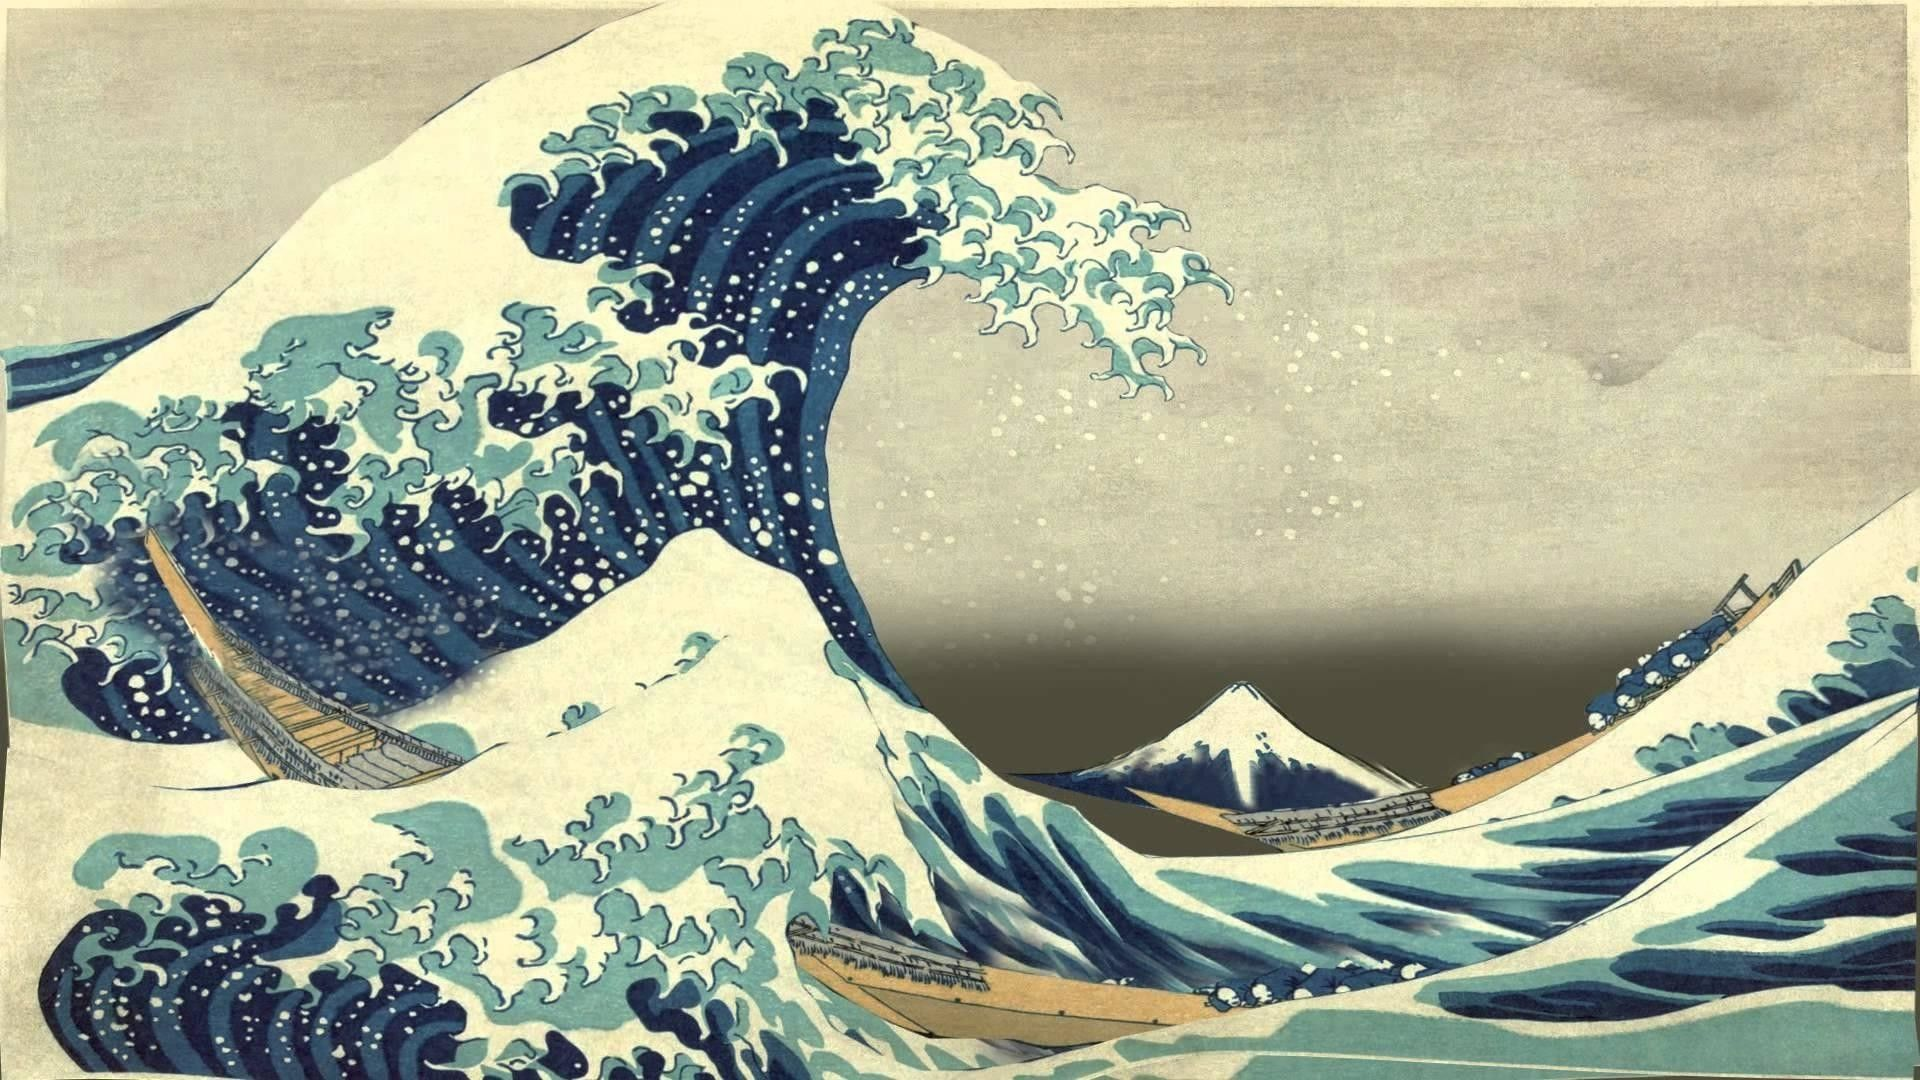
\includegraphics[width=\paperwidth]{wave.jpg}}
};
\end{tikzpicture}
\end{center}
\newgeometry{left=1.15in, right=1.15in,top=0.85in, bottom=0.85in}
    \tableofcontents
    % start lessons
    \foreach \lecno in {1,2,...,20}{%
        \edef\FileName{lectures/lecture\lecno}
        \IfFileExists{\FileName}{%
            \par
            \input{\FileName}
        }
        
    }
    
    %\chapter{Lecture 1}
\section{The Flow of Information}
% \begin{figure}
%     \centering


% \end{figure}
% \begin{tikzpicture}

% % draw rectangle node
% 	\node[draw,
% 		minimum width=2cm,
% 		minimum height=1cm,
%             fill=green!50] at (0,0){Information Source};

% % Change line color
% 	\node[draw,
%             fill=orange!50,
% 		minimum width=2cm, 
% 		minimum height=1cm,
%             shape=circle] at (3,0) {Transmuter};

% % Change filling color
% 	\node[draw,
% 		minimum width=2cm,
% 		minimum height=1cm,
%             fill=green!50] at (6,0){Channel};

% % Change text color
% 	\node[draw,
% 		text=red,
% 		minimum width=2cm, 
% 		minimum height=1cm] at (3,-2) {Process 2};

% \end{tikzpicture}

\section{Source Coding}
\begin{definition}
Given an alphabet $\Ucal$ with $|\Ucal| < \infty$. A source code $c$ is a mapping from the alphabet to the set of all finite binary strings represented as $\binset = \{null, 0, ,1, 00, 01, 10, 11, 000, \dots\}$ \ie\ $c:\Ucal \to \binset$.
\end{definition}
\begin{eg}
Consider $\Ucal = \{a,b,c,d,e\}$. Then we can have a $c:\Ucal \to \binset$ as
$c(a) = 0,$ $c(b) = 0,$ $c(c) = null,$ $c(d) = 1,$ $c(e) = 010100$.
\end{eg}
\begin{definition}
A code $c$ is called singular if $\exists u, v \in \Ucal$ s.t. $u\neq v$ but $c(u) = c(v)$.
\end{definition}
\begin{definition}
A code $c$ is called non-singular or injective if it is not singular.
\end{definition}
\begin{eg}
For the alphabet in the previous example, we can have an injective code as $c(a) = 0$, $c(b) = 00$, $c(c) = null$, $c(d) = 1$ and $c(e) = 010100$.
\end{eg}
\begin{definition}
Given $c: \Ucal \to \binset$, we write the concatenation of the codes of two letters $u_1, u_2 \in \Ucal$ as $c(u_1)c(u_2)$. We further define
\[c^2: \Ucal^2 \to \binset \text{ to be } c^2(u_1, u_2) = c(u_1)c(u_2)\]
\[c^n: \Ucal^n \to \binset \text{ to be } c^n(u_1, \dots, u_n) = c(u_1)c(u_2)\dots c(u_n)\]
\[c^*: \Ucal^* \to\binset \text{ to be } c^*(u_1,\dots,u_n) = c(u_1)c(u_2)\dots c(u_n)\]
\end{definition}
\begin{definition}
A code $c:\Ucal\to\binset$ is called uniquely decodable if $c^*$ is injective, \ie\ if $u_1,\dots,u_n \neq v_1\dots,v_k$, then $c(u_1)\dots c(u_n) \neq c(v_1)\dots c(v_k)$.
\end{definition}
\begin{eg}
With the same alphabet as before, we can have $c(a) = 0$, $c(b) = 10$, $c(c) = 110$, $c(d) = 1110$ and $c(e) = 1111$. This code is uniquely decodable and is called a prefix free code.
\end{eg}
\begin{definition}
A code $c:\Ucal\to\binset$ is called prefix free if $\forall u,v \in \Ucal$ s.t $u\neq v$, $c(u)$ is not a prefix of $c(v)$.
\end{definition}
\begin{theorem}
If a code $c$ is prefix free (p.f.), then it is uniquely decodable (u.d.).
\end{theorem}
\begin{proof}
We prove the above theorem by contradiction. Consider there exists a code $c$ which is p.f. but not u.d and we have $u_1, \dots, u_n, v_1, \dots, v_k \in \Ucal$ such that $u_1, \dots, u_n \neq v_1, \dots, v_k$ and $c(u_1)\dots c(u_n) = c(v_1)\dots c(v_k)$. Traversing the code of the sequence of alphabets from the left, we immediately notice that if $\ell(u_1) > \ell(v_1)$ then $c(v_1)$ is a prefix of $c(u_1)$. Similarly if $\ell(u_1) < \ell(v_1)$, $c(u_1)$ is a prefix of $c(v_1)$. But since the code is prefix free, we arrive at a contradiction.
\end{proof}
\begin{definition}
Given a code $c: \Ucal \to \binset$, we define the Kraft Sum
\[\ks(c) = \sum_{u \in \Ucal} 2^{-\ell(u)}\] where $\ell(u) = \text{length}(c(u))$. In case of confusion, we subscript the length by the code, i.e $\ell_c(u) \equiv \ell(u) = \text{length}(c(u))$
\end{definition}
\begin{eg}
Consider the code for the same alphabet as $c(a) = 0$, $c(b) = 1$, $c(c) = null$, $c(d) = 00$ and $c(e) = 010$. Then we have
\[
    \ks(c) = 2^{-1} + 2^{-1} + 2^0 + 2^{-2} + 2^{-2} = 2.375
\]
\end{eg}
\begin{lemma}
Suppose $c:\Ucal \to \binset$ and $d:\Vcal \to \binset$ are two codes, and denote $(c\times d): \Ucal \times \Vcal \to \binset$ as $(c\times d)(u,v) = c(u)d(v)$. Then 
\[\ks(c\times d) = \ks(c)\ks(d)\]
\end{lemma}
\begin{proof}
By definition, we have
\begin{align*}
    \ks(c\times d) &= \sum_{u,v} 2^{-\ell_{c\times d}((u,v))} = \sum_{u,v} 2^{-[\ell_c(u) + \ell_d(v)]} \\
    &= \sum_{u,v} 2^{-\ell_c(u)} \times 2^{-\ell_d(v)} = \sum_u 2^{-\ell_c(u)} \sum_v 2^{-\ell_d(v)} = \ks(c)\ks(d)
\end{align*}
\end{proof}
\begin{corollary}
$\ks(c^n) = [\ks(c)]^n$
\end{corollary}
\begin{theorem}[Kraft's Inequalities]
Suppose $c: \Ucal \to \binset$ is injective, then
\[\ks(c) \leq \log_2(1+|\Ucal|)\]
Suppose $c$ is uniquely decodable, then
\[\ks(c) \leq 1\]
Suppose $c$ is prefix free, then
\[\ks(c) \leq 1\]
\end{theorem}
\begin{proof}
Suppose that $c$ is injective, and let $|\Ucal| = k$ and $\Ucal = \{1, 2, \cdots, k\}$. To maximize the Kraft Sum, we put $c(1) = null$, $c(2) = 0$, $c(3) = 1$ and so on. Also, let $k = 1 + 2 + 4 + 8 + \cdots + 2^{m-1} + r$ where $0 \leq r < 2^m$. Then, we can write
\[\ks(c) = 2 + 2 \times 2^{-1} + 2^2 \times 2^{-2} + \cdots + 2^{m-1}\times 2^{-(m-1)} + r \times 2^{-m} = m + r \cdot 2^{-m}\]
Now, consider $\log_2(1+k) = \log_2(1 + 2^{m} - 1 + r) = \log_2(2^m + r)$. We can then write \[\log_2(1+k) \leq \log_2(2^m(1+r\cdot2^{-m})) = m + \log_2(1+r\cdot 2^{-m}) \]
Notice that $r\cdot 2^{-m} \in [0,1)$ and using the fact that $\log_2(1+x) \geq x$ for $x\in[0,1]$, we get
\[m + \log_2(1+r2^{-m}) \geq m + r\cdot2^{-m} = \ks(c)\]
Having proved for $c$ being injective, we now show it for $c$ being uniquely decodable. First observe that $c$ is u.d. $\iff$ $c^*$ is injective $\implies \forall n,$ $c^n$ is injective. Hence, we can write
\[
[\ks(c)]^n = \ks(c^n) \leq \log_2(1+k^n)
\]
Now, notice that the LHS is exponentially growing in $\ks(c)$ while the RHS is linearly growing in $\ks(c)$. Since exponential growth cannot be dominated by linear growth, we notice that the term growing exponentially must be less than or equal to 1. Thus, we have $\ks(c) \leq 1$.

\noindent
Finally, since every prefix free code is uniquely decodable, the last inequality follows immediately.
\end{proof}
\begin{remark}
Although the Kraft Sum for uniquely decodable codes is less than or equal to 1, the reverse doesn't hold true. Take the code $\Ucal = \{a,b,c\}$ and the code $c$ to be $c(a) = 0$, $c(b) = 00$ and $c(c) = 00$. It is clear that $c$ is not uniquely decodable, but --
\[
\ks(c) = 2^{-1} + 2^{-2} + 2^{-2}  = 1 \leq 1
\]
\end{remark}
    % end lessons
\end{document}